\pagebreak

\section{Результаты}
\textbf{Примеры работы программы:}
\begin{center}
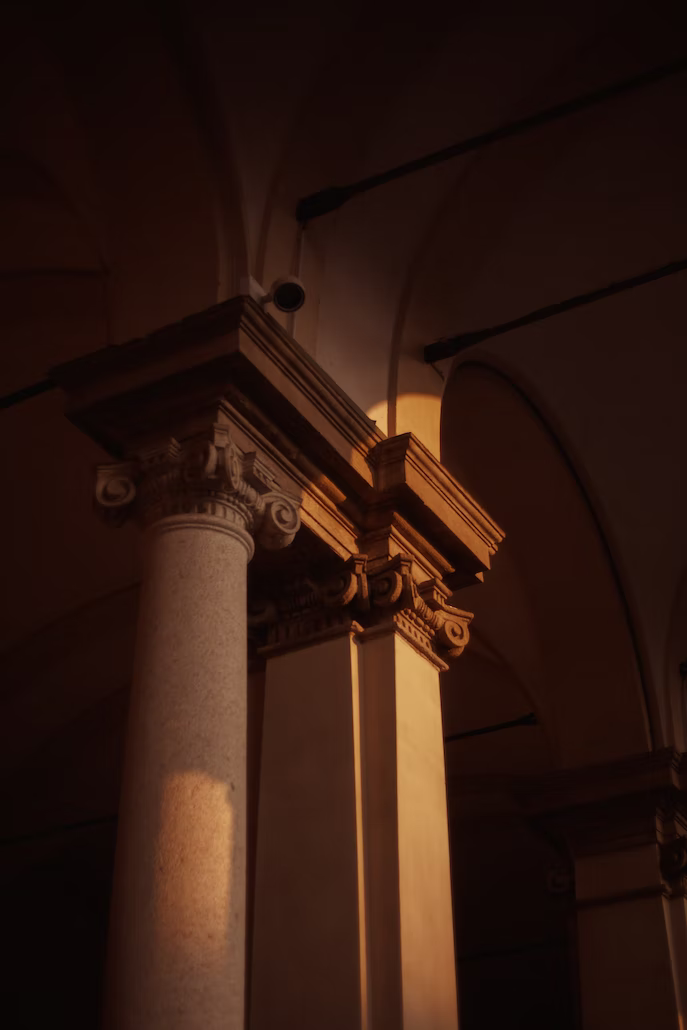
\includegraphics[width=.49\textwidth]{pillars}\hfill
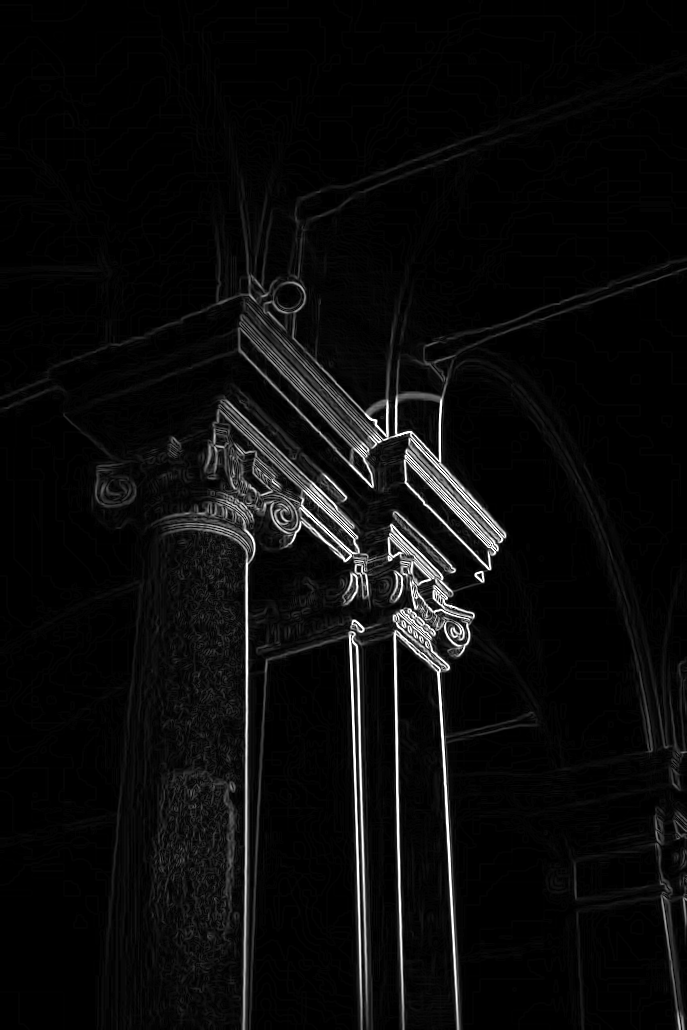
\includegraphics[width=.49\textwidth]{pillars_edges}

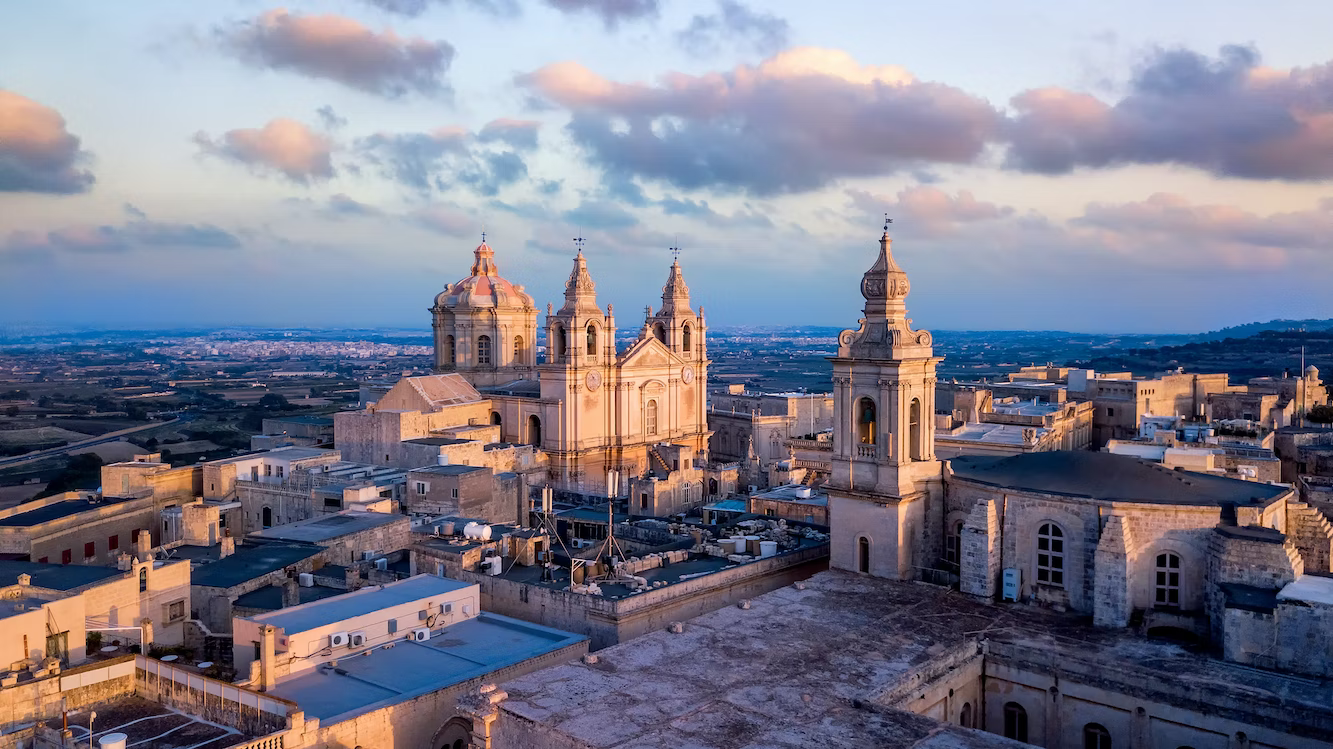
\includegraphics[width=.49\textwidth]{cathedral}\hfill
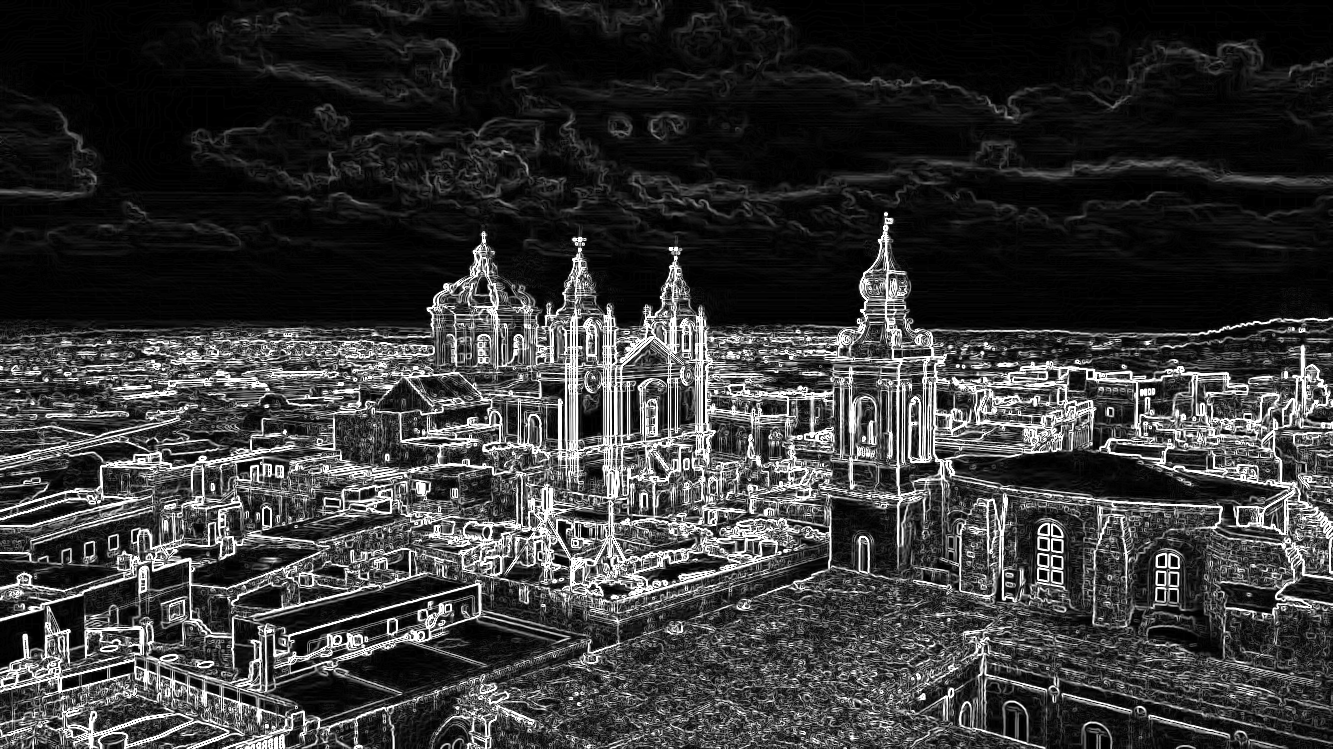
\includegraphics[width=.49\textwidth]{cathedral_edges}

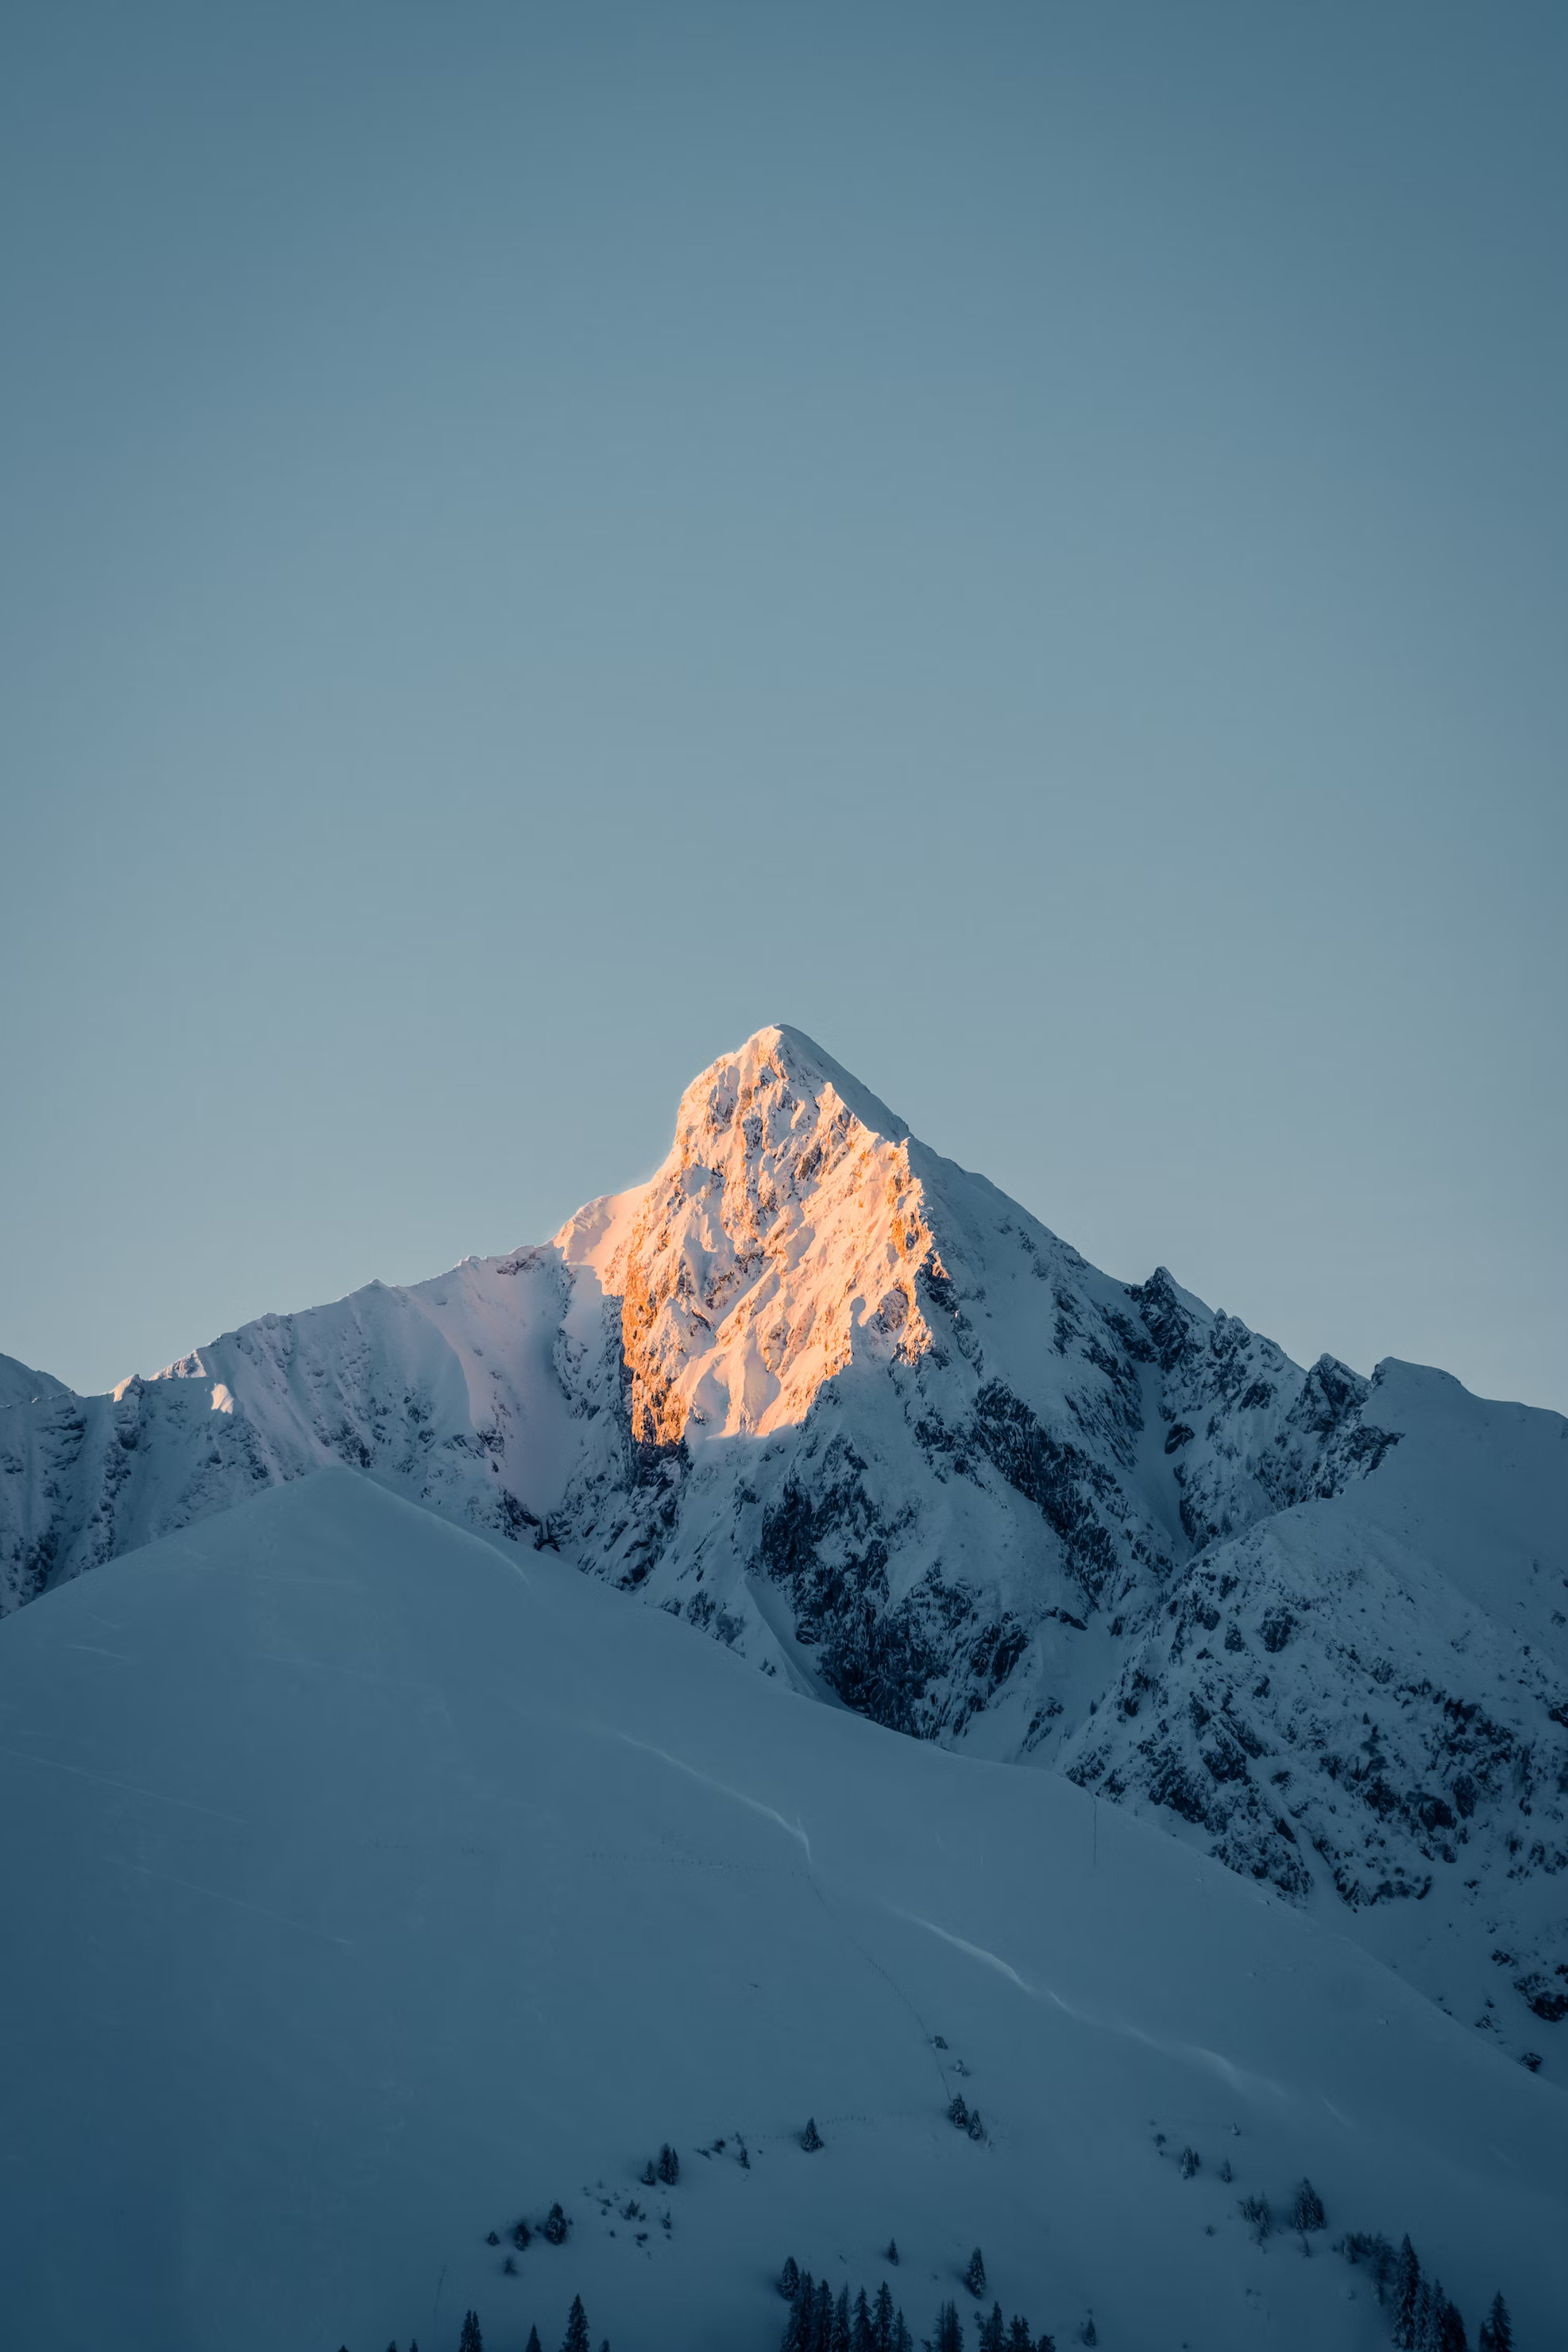
\includegraphics[width=.49\textwidth]{mountain}\hfill
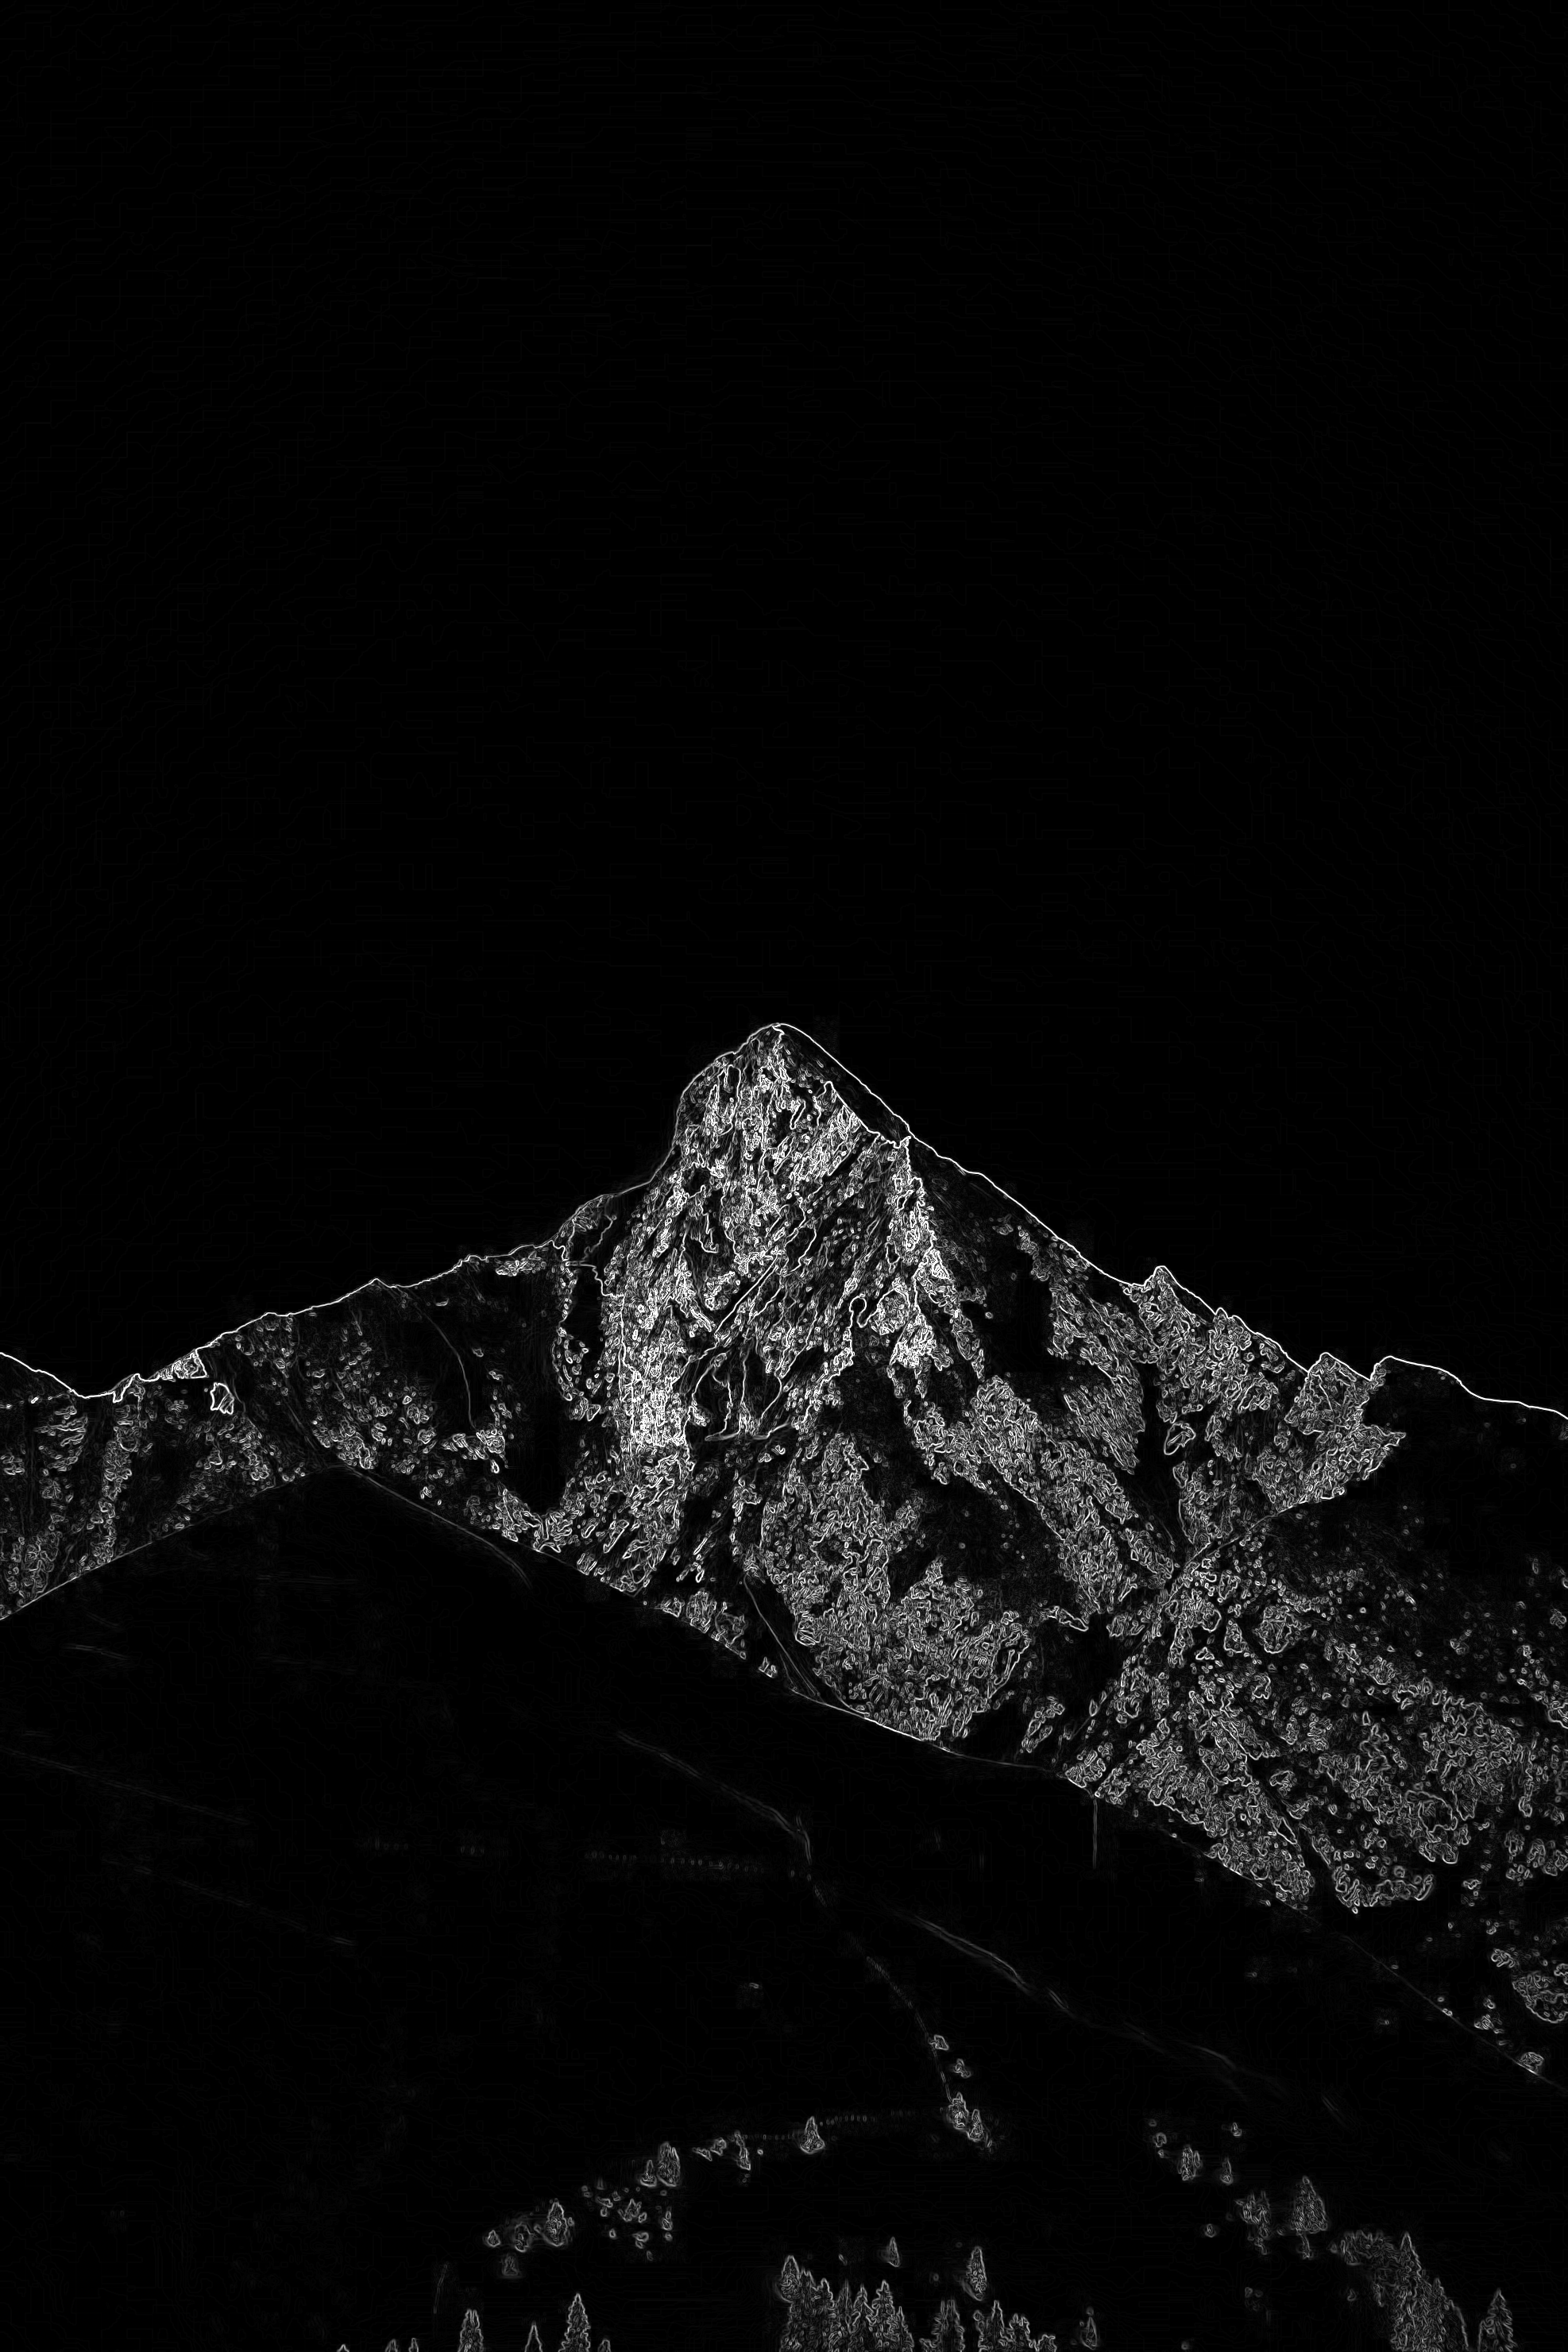
\includegraphics[width=.49\textwidth]{mountain_edges}

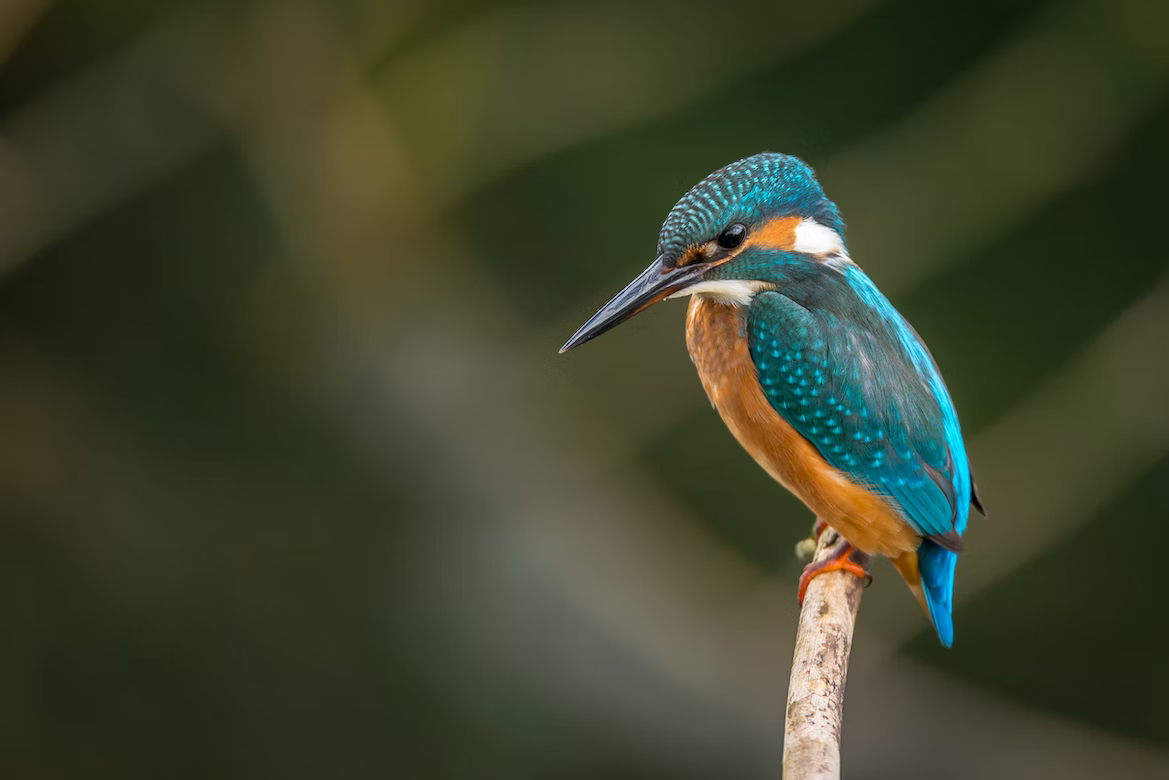
\includegraphics[width=.49\textwidth]{kingfisher}\hfill
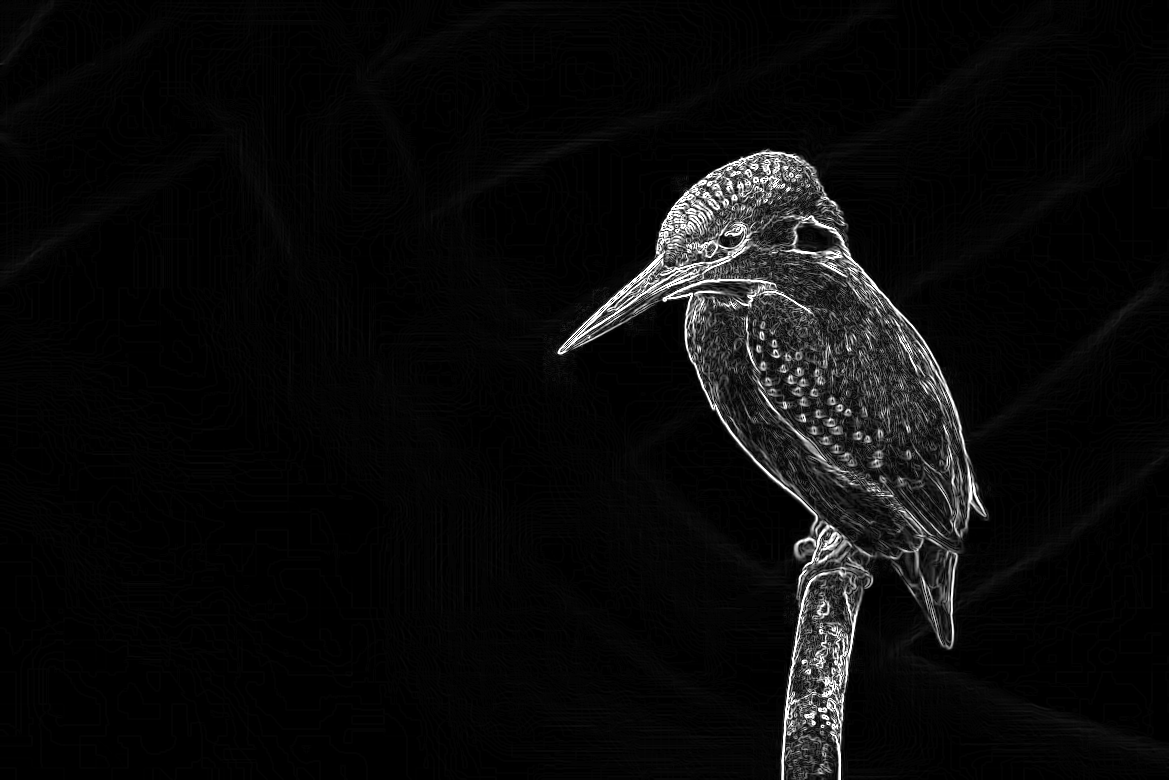
\includegraphics[width=.49\textwidth]{kingfisher_edges}
\end{center}

\textbf{Сравнение времени работы:}
\begin{center}
\begin{tabular}{|l*{5}{|r}|}
\hline
\textbf{Конфигурация} & \multicolumn{5}{c|}{\textbf{Время выполнения, мс}} \\
\hline
CPU            &   1.902230 &  48.822700 &   202.029000 &   819.271000 &  5135.030000 \\
\hline
1$\times$1, 32$\times$1      &   0.627040 &  12.253200 &    65.633900 &   215.664000 &  1238.230000 \\
\hline
1$\times$1, 32$\times$32     &   0.183968 &   3.098140 &    15.405900 &    47.854300 &   302.103000 \\
\hline
32$\times$32, 32$\times$8    &   0.114176 &   0.774368 &     2.823550 &     9.764260 &    60.597000 \\
\hline
32$\times$32, 32$\times$32   &   0.155936 &   0.971296 &     3.378780 &    10.265200 &    61.083200 \\
\hline
64$\times$64, 32$\times$8    &   0.200288 &   1.184830 &     3.285180 &    10.160500 &    60.955600 \\
\hline
64$\times$64, 32$\times$32   &   0.356704 &   1.397250 &     4.145730 &    12.191700 &    63.058200 \\
\hline
128$\times$128, 32$\times$8  &   0.425472 &   1.819140 &     5.060800 &    11.851400 &    62.656300 \\
\hline
128$\times$128, 32$\times$32 &   1.035650 &   2.492030 &     5.967460 &    15.019600 &    71.128200 \\
\hline
\textbf{Размер теста} & 100x100 & 500x500 & 1000x1000 & 2000x2000 & 5000x5000 \\
\hline
\end{tabular}
\end{center}
